% !TEX program = xelatex
\documentclass{CSUthesis}


\usepackage[figure,table]{totalcount}
\usepackage{totcount}

%参考文献计数
\newtotcounter{citnum}
\def\oldbibitem{} \let\oldbibitem=\bibitem
\def\bibitem{\stepcounter{citnum}\oldbibitem}
%\total{citnum}
%累积引用次数计数
%\newtotcounter{citesnum}/
%\def\oldcite{} \let\oldcite=\cite
%\def\cite{\stepcounter{citesnum}\oldcite}
%\total{citesnum}

%%%%%%%%%%%%%%%%%%%%%%%%%%%%%%%%%%%%%%%%%%%%%%%%%%
% 前置部分的页眉页脚设置
% -----------------------------------------------%
% 正文和后置部分用阿拉伯数字编连续码,前置部分用罗马数字单独编连续码(封面除外)。
% 设置封面页后的页码

% 设置页眉和页脚 
\pagestyle{fancy}
% 正文以前部分无需页眉
\fancyhf{} % 清空原有格式
\renewcommand{\headrulewidth}{0pt}
% 中文摘要之前无需页码

%!TEX root = ../csuthesis_main.tex
% 文章信息
\titlecn{数据驱动的互联网卡用户离网预测及干预算法研究}
\titleen{中南大学 \\Central South University}

\priormajor{计算机科学与技术}
\minormajor{计算机应用技术}
\interestmajor{深度学习}
\author{钱凯}
\supervisor{吕丰\ 教授}
\subsupervisor{}
\department{计算机学院}
\studentid{144601044}
\thesisdate{year=2022,month=4}



\clcnumber{TP391} 				% 中图分类号 Chinese Library Classification
\schoolcode{10533}			% 学校代码
\udc{004.9}						% UDC
\academiccategory{学术学位}	% 学术类别


\newif \ifblindreview % 条件语句,是否是盲审版本
\newif \ifAcademic % true为学术学位,false为专业学位
\newif \ifPublic   % true为公开,false为涉密
\newif \ifDoctor   % 是否为博士学位论文



%\blindreviewtrue  %%盲审版本
\blindreviewfalse  %%正常版本

\Academictrue % 学术学位
%\Academicfalse % 专业学位

\Publictrue  % 公开
%\Publicfalse % 涉密

%\Doctortrue  % 博士学位论文
\Doctorfalse % 硕士学位论文




\begin{document}
	%%%%%%%%%%%%%%%%%%%%%%%%%%%%%%%%%%%%%%%%%%%%%%%%%%
	% 封面
	% -----------------------------------------------%
	\makecoverpage
	
	\clearpage
	\mbox{}
	\clearpage
	
%	\ifblindreview	% 盲审不需要扉页和声明页
%	\else
	%%%%%%%%%%%%%%%%%%%%%%%%%%%%%%%%%%%%%%%%%%%%%%%%%%
	% 扉页 
	% -----------------------------------------------%
	
	\maketitlepage
	
	\clearpage
	\mbox{}
	\clearpage
	
	\setlength{\headheight}{9.6mm}
	\setlength{\footskip}{7.9mm}
	\setlength{\textheight}{681.5pt} % 调整版面高度
	%%%%%%%%%%%%%%%%%%%%%%%%%%%%%%%%%%%%%%%%%%%%%%%%%%
	% 声明页
	% -----------------------------------------------%
	\announcement
	\clearpage
	\mbox{}
	\clearpage
%	\fi
	%%%%%%%%%%%%%%%%%%%%%%%%%%%%%%%%%%%%%%%%%%%%%%%%%%
	
	% 设置页眉和页脚 %
	\setlength{\headheight}{9.6mm}
	\setlength{\footskip}{7.9mm}
	\pagestyle{fancy}
	\fancyhf[CF]{\TimesNewRoman \zihao{-5} \thepage} % 所有(奇数和偶数)中间页脚,TimesNewRoman小五号
	
	\addtocontents{toc}{\vspace{-8pt}}
	
	% 中文摘要
	% -----------------------------------------------%
	\pagenumbering{Roman} % 重摘要至目录部分页码为大写罗马字体
	\setcounter{page}{1} % 页码从I重新开始
	\phantomsection                %% 解决目录中超链接地址错误问题
	\addcontentsline{toc}{section}{摘要} %%增加摘要至目录且与第一章对齐
	%!TEX root = ../csuthesis_main.tex
% 设置中文摘要
\keywordscn{离网预测;用户偏好;用户干预;深度学习;强化学习}
\categorycn{TP391}
\itemcountcn{图 \totalfigures\ 幅,表 \totaltables\ 个,参考文献 \total{citnum}\ 篇}

\begin{abstractcn}\setlength{\baselineskip}{20pt}%\renewcommand{\baselinestretch}{1.0}
	
	互联网卡是最近通信运营商和互联网公司合作提出的一种新的商业模式,可以享受由合作互联网公司应用产生流量费用的大幅折扣或减免。然而,因为中国互联网卡市场竞争日趋激烈,需求逐步饱和等多种原因,用户离网/流失问题也日益严重,造成了较大的经济损失。为了全流程自动化高效地挽留住用户,本文针对互联网卡用户离网预测、离网原因推断和用户挽留问题展开研究。但是,要解决这些问题存在以下三个挑战:
	\par
	1) 通信运营商的互联网卡用户规模较大,分布全国各地,异构特征显著,数据类型丰富,速度增长快,因此如何精准且全面地预测出其中潜在的离网用户成为了一个十分重要的挑战。\par
	2) 互联网卡用户的离网原因高达上百种且只有少部分的离网用户有记录离网原因,如何在少量标注数据的情况下,如何合理、高效地表征用户离网偏好成为了一个棘手的挑战。\par
	3) 由于缺乏用户干预交互记录,并且通信运营商等企业在实际干预过程中给予的预算往往是有限的。因此如何向预离网用户匹配合适的挽留措施,既能解决用户使用过程中的痛点,同时又不会让企业方付出过高的成本是一个极大的挑战。\par
	为解决上述挑战,本文设计一种用户偏好感知的挽留框架(\emph{UPRF},\underline{U}ser \underline{P}reference-Aware \underline{R}etention \underline{F}ramework),具体而言,\emph{UPRF}框架包含以下三部分内容:\par
	1)基于自注意力机制的互联网卡用户离网预测模块。首先对离网行为等做了详细的数据分析,接着从用户数据中分别提取了用户画像特征和序列特征,最后设计和实现了一种融合主成分分析算法和自注意力机制的互联网卡用户离网预测模型。	\par
	2)基于排名加权归一化技术的离网偏好表征模块。首先抽取了5类能够被数据反映的离网原因,其次挑选了与这些离网原因相关的偏好特征,接着设计并实现了基于等频分箱的双重排名离散化算法,得到原始离网偏好向量,
	%然后通过不可信用户过滤机制排除了不活跃的预离网用户,
	最后使用用户自适应权重归一化算法表征预离网用户的离网偏好。		         \par
	3)资源有限上下文的用户偏好感知挽留策略匹配模块。首先将挽留策略匹配问题建模成多臂老虎机问题,然后接收由上述模块给出的离网风险和离网偏好,使用基于领域知识的分布初始化奖励生成模型,最后训练基于资源有限上下文的偏好感知的挽留策略匹配算法。	
	\par
	最后,大量数据驱动的实验表明\emph{UPRF}框架可以精准全面地预测潜在离网用户,有效提高挽留用户数和运营商收入总和。与最好的基准模型对比,其分别提升了12\%,25\%和23\%。此外,大量的健壮性测试也表明\emph{UPRF}框架在不同参数设置的情况下都具有较好的性能表现。	
%	由此,本文针对互联网卡用户离网预测和干预挽留问题展开研究。首先,离网预测问题和挽留策略匹配问题分别被形式化建模为二分类和多臂老虎机问题,并且以最大化挽留成功离网用户数为优化目标。
%然后考虑到运营商互联网卡用户数据规模较大,异构特征显著等挑战,需要一种高效,精准和全面的互联网卡用户干预框架,这对于互联网卡用户维系而言至关重要。	
%	互联网卡是最近通信运营商和互联网公司合作提出的一种新的商业模式,可以享受由合作互联网公司应用产生流量费用的大幅折扣或减免。然而因为中国互联网卡市场竞争日趋激烈,需求逐步饱和,用户离网问题也日益严重,造成了较大的经济损失。
%	为此,本文设计一种用户偏好感知的挽留框架(UPRF,\underline{U}ser \underline{P}reference-Aware \underline{R}etention \underline{F}ramework),通过数据驱动的方式对互联网卡用户进行离网预测,然后基于排名归一化技术表征离网偏好,最后结合强化学习算法对预离网用户进行挽留策略匹配。具体而言,UPRF框架包含以下三部分内容:
%		\par
%%\begin{enumerate}[label=\arabic*)]	
%%	\item 
%	1)融合主成分分析算法和自注意力机制的互联网卡用户离网预测模块。%设计与实现
%	针对运营商互联网卡的用户数据规模较大,异构特征显著等挑战,本文对离网行为等做了详细的数据分析,
%	接着从用户数据中分别提取了用户静态画像特征和序列特征,
%	最后设计和实现了一种融合主成分分析算法和自注意力机制的互联网卡用户离网预测模型,
%	以在月初向运营商输出当月的潜在离网用户名单和对应的离网风险值列表。
%	\par
%%	\item 
%	2)基于排名加权归一化技术的离网偏好生成模块。
%	针对互联网卡用户离网原因众多和往往因为多个原因的叠加而发生离网行为等挑战,
%	本文首先抽取了5个能够被数据反映的离网原因,
%	其次挑选了与这些离网原因较为相关的偏好特征,
%	接着设计并实现了基于等频分箱的双重排名离散化算法,
%	得到预离网用户的原始离网偏好向量,
%	然后通过不可信用户过滤机制排除了不活跃的预离网用户,
%	最后使用用户自适应权重归一化算法向运营商和挽留策略匹配模块输出预离网用户的离网偏好。		
%	\par
%%	\item 
%	3)资源有限上下文的用户偏好感知挽留策略匹配模块。
%	针对由于现阶段运营商营销部门预算有限,
%	无法通过较低的挽留成本将预离网用户留存下来等问题,
%	本文首先对挽留策略匹配问题建模成多臂老虎机问题,
%	然后接收由互联网卡用户离网预测模块给出的离网风险值和互联网卡预离网用户离网偏好生成模块给出的离网偏好,
%	使用基于领域知识的分布初始化奖励生成模型,
%	最后训练基于资源有限上下文的偏好感知的挽留策略匹配算法。		
%	\par
%%\end{enumerate}			
%	最后,大量数据驱动的实验表明UPRF框架可以精准全面地预测潜在离网用户,有效提高挽留用户数和运营商收入总和。与最好的基准模型对比,其分别提升了12\%,25\%和23\%。此外,大量的健壮性测试也表明UPRF框架在不同参数设置的情况下都具有较好的性能表现。
%LaTeX利用设置好的模板,可以编译为格式统一的pdf。目前国内大多出版社与高校仍在使用word,word由于其强大的功能与灵活性,在新手面对形式固定的论文时,排版、编号、参考文献等简单事务反而会带来很多困难与麻烦,对于一些需要通篇修改的问题,要想达到LaTeX的效率,对word使用者来说需要具有较高的技能水平。
%
%为了能把主要精力放在论文撰写上,许多国际期刊和高校都支持LaTeX的撰写与提交,新手不需要关心格式问题,只需要按部就班的使用少数符号标签,即可得到符合要求的文档。且在需要全篇格式修改时,更换或修改模板文件,即可直接重新编译为新的样式文档,这对于word新手使用word的感受来说是不可思议的。
%
%本项目的目的是为了创建一个符合中南大学研究生学位论文(博士)撰写规范的TeX模板,解决学位论文撰写时格式调整的痛点。
\end{abstractcn}
	\clearpage
	
	%%%%%%%%%%%%%%%%%%%%%%%%%%%%%%%%%%%%%%%%%%%%%%%%%%
	% 英文摘要
	% -----------------------------------------------%
	\phantomsection                %% 解决目录中超链接地址错误问题
	\addcontentsline{toc}{section}{ABSTRACT}
	%!TEX root = ../csuthesis_main.tex
\keywordsen{Churn Prediction; User Preference; User Intervention; Deep Learning; Reinforcement Learning}
\categoryen{TP391}
%\itemcountcn{There are \totalfigures\ figures, \totaltables\ tables, and \total{citnum}\ citations in this thesis.}
%\addcontentsline{toc}{section}{ABSTRACT}
\begin{abstracten}\setlength{\baselineskip}{20pt}
	
	Internet card (IC) is a new business model proposed recently by the cooperation of cellular operators and Internet companies. Particularly, IC users can enjoy significant discounts or exemptions on target traffic budget, that generated by the applications of partner Internet companies.However, in China, because of the market of IC is becoming increasingly competitive, the demand of IC is gradually saturated, etc., the churn problem of IC user is getting worse which led to much economic loss. In order to automatically and efficiently retain users throughout the entire process, this paper conducts research on the churn prediction and the churn reason inference of Internet card users and the retention issues. Nevertheless, there are three challenges to addressing these issues:\par
	1)The Internet card users of communication operators are relatively large, distributed all over the country, with obvious heterogeneous characteristics, rich data types and fast growth. Therefore, how to predict potential churner of IC accurately and comprehensively has become a significant challenge.\par
	2)There are hundreds of reasons for Internet card users to churn, and only a few users have recorded the reasons for churning. How to reasonably and efficiently represent the user’s churn preference with a small amount of labeled data has become a thorny challenge.\par
	3)Due to the lack of user intervention interaction records, and the budget given by companies such as communication operators in the actual intervention process is often limited. Therefore, how to match appropriate retention measures to pre-churners can not only solve the problems in the user's use process, but at the same time not make the enterprise pay too much cost is a great challenge.\par
	To address these issues, we proposed a \underline{U}ser \underline{P}reference-Aware \underline{R}etention \underline{F}ramework. Specifically, the \emph{UPRF} framework includes the following three parts:
	\par
	1) Internet card churn prediction module based on self-attention mechanism.
	We firstly makes a detailed data analysis on churn behavior, churn reason, etc. Then, the IC user's portrait features and sequence features are extracted from the user data respectively. Finally, an Internet card user churn prediction model that combines principal component analysis algorithm and self-attention mechanism is designed and implemented.	
%	to output the list of potential churn users and the corresponding churn risk value list of the current month to the operator at the beginning of the month.
	\par
	2) Churn preference generation module based on ranking-weighted normalization technology. We firstly extracts 5 churn reasons that can be reflected by the data. Secondly, the preference characteristics that are more related to these churn reasons are selected. Then, a dual ranking discretization algorithm based on equal frequency binning was designed and implemented to present raw churn preference of pre-churners. Finally, the user-adaptive weight normalization algorithm is used to output the churn preference of the pre-churners.
	\par
	3) User preference-aware retention strategy matching module in a resource-limited contexts.	The retention strategy matching problem is firstly modeled as a multi-armed bandit problem. Then the strategy matching module receives the churn risk value given by the churn prediction module and the churn preference given by the churn preference generation module. Nextly, it initializes the reward generation model using a distribution based on domain knowledge. Finally, a preference-aware retention strategy matching algorithm in a resource-limited context is trained.
	\par
	Last but not least, extensive data-driven experiments demonstrate the efficacy of \emph{UPRF} in predicting potential IC churner and raising number of reserved user and total revenue of mobile commnications operator. Comparing to the best benchmark models, it imporved by 12\%, 25\% and 23\%, respectively. Furthermore, comprehensive robustness testing shows that \emph{UPRF} has good perfermance under different parameter settings.	
	
%Internet card (IC) is a new business model proposed recently by the cooperation of cellular operators and Internet companies. Particularly, IC users can enjoy significant discounts or exemptions on target traffic budget, that generated by the applications of partner Internet companies. However, in China, the market of IC is becoming increasingly competitive, the demand of IC is gradually saturated, the churn problem of IC user is getting worse which led to much economic loss. To address these issues, we proposed a \underline{U}ser \underline{P}reference-Aware \underline{R}etention \underline{F}ramework, named UPRF. It utilizes a data-driven approach, ranking-weighted normalization technology and reinforcement learning to predict potential churner, represent churn preference, match retention strategy, respectively. Specifically, the UPRF framework includes the following three parts:
%\par
%1) Internet card churn prediction module integrating principal component analysis algorithm and self-attention mechanism.
%In view of the challenges of large-scale user data and significant heterogeneous characteristics of the Internet card of the operator, this paper makes a detailed data analysis on churn behavior, churn reason, etc. Then, the IC user's static portrait features and sequence features are extracted from the user data respectively. Finally, an Internet card user churn prediction model that combines principal component analysis algorithm and self-attention mechanism is designed and implemented to output the list of potential churn users and the corresponding churn risk value list of the current month to the operator at the beginning of the month.
%\par
%2) Churn preference generation module based on ranking-weighted normalization technology. In view of the challenges of massive churn reasons of IC users and of IC users often churning due to multiple reasons, the paper first extracts 5 churn reasons that can be reflected by the data. Secondly, the preference characteristics that are more related to these churn reasons are selected. Then, a dual ranking discretization algorithm based on equal frequency binning was designed and implemented to present raw churn preference of pre-churners. Then the inactive pre-churners are excluded through the untrustworthy user filtering mechanism. Finally, the user-adaptive weight normalization algorithm is used to output the churn preference of the pre-churners to the operator and the retention strategy matching module.
%\par
%3) User preference-aware retention strategy matching module in a resource-limited contexts.
%Due to the limited budget of the marketing department of operators, problems merged such as the inability to retain pre-churners through low retention costs. In this paper, the retention strategy matching problem is firstly modeled as a multi-armed bandit problem. Then the strategy matching module receives the churn risk value given by the churn prediction module and the churn preference given by the churn preference generation module. Nextly, it initializes the reward generation model using a distribution based on domain knowledge. Finally, a preference-aware retention strategy matching algorithm in a resource-limited context is trained.
%\par
%Last but not least, extensive data-driven experiments demonstrate the efficacy of UPRF in predicting potential IC churner and raising number of reserved user and total revenue of mobile commnications operator. Comparing to the best benchmark models, it imporved by 12\%, 25\% and 23\%, respectively. Furthermore, comprehensive robustness testing shows that UPRF has good perfermance under different parameter settings.

	
%Internet card is a new business model recently proposed by mobile communication operators and internet companies in cooperation. It allows users to enjoy significant discounts or exemptions on the target traffic budget generated by cooperating internet companies. However, due to the increasingly fierce competition in the Chinese internet card market, demand is gradually saturating, and the problem of user churn is becoming more serious, resulting in significant economic losses. Therefore, this article focuses on predicting and intervening to retain internet card users.
%
%Firstly, the problem of user churn prediction and intervention strategy matching are formally modeled as binary classification and sequence decision problems, respectively, with maximizing the number of successfully retained users as the optimization objective. Then, considering the challenges of large-scale heterogeneous features of internet card user data, a significant framework for efficient, accurate, and comprehensive internet card user intervention is proposed, which is crucial for maintaining internet card users.
%
%To this end, this article designs a \underline{U}ser \underline{P}reference-Aware \underline{R}etention \underline{F}ramework (UPRF) that predicts internet card user churn in a data-driven manner, characterizes churn preferences based on weighted normalization techniques, and combines reinforcement learning algorithms to match intervention strategies for potential churn users. Specifically, the UPRF framework includes the following three parts:
%
%1) Design and implementation of an internet card user churn prediction module that integrates principal component analysis algorithm and self-attention mechanism.
% Considering the challenges of large-scale heterogeneous features of internet card user data, this article conducts detailed data analysis on churn behavior, extracts static portrait features and sequence features from user data, and finally designs and implements an internet card user churn prediction model that integrates principal component analysis algorithm and self-attention mechanism. At the beginning of each month, the model outputs a list of potential churn users and corresponding churn risk values to the operator.\par
%2) Design and implementation of a churn preference generation module based on rank-weighted normalization techniques. 
%Considering the challenges of multiple reasons for internet card user churn and the tendency for churn behavior to be a result of a combination of factors, this article first extracts five churn reasons that can be reflected in the data. Then, the relevant preference features are selected and a ranking normalization algorithm based on equi-frequency binning is designed and implemented. The raw churn preference vector of predicted churn users is obtained, and inactive predicted churn users are filtered out using an untrustworthy user filtering mechanism. Finally, the churn preference representation of predicted churn users is output to the operator and intervention strategy matching module using a user adaptive weighting normalization algorithm.\par
%3) Design and implementation of the user preference-aware intervention strategy matching module with limited resources context.
% In response to the challenges of crude retention measures designed by the marketing departments of telecom operators at present, which cannot retain potential churn users at low retention costs, this article first models the intervention strategy matching problem as a sequential decision problem. Then, it receives the churn risk values given by the Internet card user churn prediction module and the churn preference given by the Internet card pre-churn user churn preference generation module. It uses a domain-knowledge-based distribution initialization reward generation model and finally trains the preference-aware intervention strategy matching algorithm based on limited resource context.\par
%Finally, a large amount of data-driven experiments show that the UPRF framework can effectively increase the number of retained users and the total revenue of the telecom operator. In addition, a large number of robustness tests also show that the UPRF framework has good robustness under different parameter settings.

\end{abstracten}

	\clearpage
	
	% 目录
	% -------------------------------------------%
	{
		\renewcommand*{\baselinestretch}{1.3841}   % 行间距20pt
		\renewcommand{\contentsname}{\vspace{10pt} \hfill \heiti \bfseries \zihao{3} 目\quad 录\hfill ~\\}
		\phantomsection                %% 解决目录中超链接地址错误问题
		\addcontentsline{toc}{section}{目录} % 在目录中添加目录页码.
		\tableofcontents
	}
	\clearpage
	
	% 插图索引
	% -------------------------------------------%
	{
		\setlength{\baselineskip}{20pt}         % 基准行间距
		\renewcommand{\baselinestretch}{1.0}   % 几倍行间距
		{~}
		\vspace{-10pt}
		\renewcommand{\listfigurename}{\hfill \heiti \zihao{3} 插图索引\hfill ~\\}  
		% 在目录中添加插图索引页码,按需确定是否注释下面两行
		\phantomsection                %% 解决目录中超链接地址错误问题
		\addcontentsline{toc}{section}{插图索引} 
		%%设置插图索引的 图 标签
		\let\oldnumberline\numberline%
		\renewcommand{\numberline}{\figurename~\oldnumberline}
		%增加图目录,按需确定是否注释下面一行
		\listoffigures
	}
	
	\clearpage
	
	% 表格索引
	% -------------------------------------------%
	{
		\setlength{\baselineskip}{20pt}         % 基准行间距
		\renewcommand{\baselinestretch}{1.0}   % 几倍行间距
		{~}
		\vspace{-10pt}
		\renewcommand{\listtablename}{\hfill \heiti \zihao{3} 表格索引\hfill ~\\}  
		% 在目录中添加表格索引页码,按需确定是否注释下面两行
		\phantomsection                %% 解决目录中超链接地址错误问题
		\addcontentsline{toc}{section}{表格索引}
		%%设置表格索引的 表 标签
		\let\oldnumberline\numberline%
		\renewcommand{\numberline}{\tablename~\oldnumberline}
		%增加表目录,按需确定是否注释下面一行
		\listoftables
	}
	
	\clearpage
	
	
	%%%%%%%%%%%%%%%%%%%%%%%%%%%%%%%%%%%%%%%%%%%%%%%%%%
	% 符号说明(必要时)
	% -----------------------------------------------%
%	\phantomsection                %% 解决目录中超链接地址错误问题
%	\addcontentsline{toc}{section}{符号说明} % 在目录中添加目录页码.
%	%\begin{denotation}
%\songti \zihao{5}
%%\songti \zihao{5}
%\begin{center}%此处最好是h
%\arrayrulewidth1pt
%\resizebox{\textwidth}{!}{
%\begin{tabular}{| m{0.4\textwidth}<{\centering} | m{0.3\textwidth}<{\centering} | m{0.3\textwidth}<{\centering} |}
%\hline
%符号&意义&单位(量纲)\\
%\hline
%频率&赫[兹]&Hz\\
%\hline
%\end{tabular}}
%\end{center}
%\end{denotation}

	
	%%%%%%%%%%%%%%%%%%%%%%%%%%%%%%%%%%%%%%%%%%%%%%%%%%
	% 正文页眉页脚
	% -----------------------------------------------%
	
	\renewcommand{\headrulewidth}{1pt}
	
	% 去掉页眉章节序号后面的“.”
	\renewcommand{\sectionmark}[1]{\markboth{第{\thesection}章~ #1}{第{\thesection}章~ #1}}
	\renewcommand{\subsectionmark}[1]{\markright{\leftmark}}
	\renewcommand{\subsubsectionmark}[1]{\markright{\leftmark}}
	
	\fancyhf[RH]{\songti \zihao{5} \leftmark} % 设置所有(奇数和偶数)右侧页眉net
	\ifDoctor
	\fancyhf[LH]{\songti \zihao{5} 中南大学博士学位论文} % 设置所有(奇数和偶数)左侧页眉
	\else
	\fancyhf[LH]{\songti \zihao{5} 中南大学硕士学位论文} % 设置所有(奇数和偶数)左侧页眉
	\fi
	% 正文内容 
	% --------------------------------------------%
	\setcounter{page}{1} % 重置页码编号
	\pagenumbering{arabic} % 设置页码编号为阿拉伯数字
	
	% 可以使用include命令导入tex文件,从而避免过多修改本文件。
	
	% 论文正文是主体,主体部分应从另页右页开始,每一章应另起页。一般由序号标题、文字叙述、图、表格和公式等五个部分构成。
	
	% 重新设置正文行间距,因为前置部分设置时候行间距被改过
	\renewcommand*{\baselinestretch}{1.0}   % 几倍行间距
	\setlength{\baselineskip}{20pt}         % 基准行间距
	
	% 正文
	{
		% 表格字号应比正文小,一般五号/10.5pt,但是暂时没法再cls里设置(不然会影响到封面等tabular环境)
		% 所以目前只好在主文件里局部\AtBeginEnvironment
		\AtBeginEnvironment{tabular}{\zihao{5}}
		%!TEX root = ../csuthesis_main.tex
% 论文正文是主体,主体部分应从另页右页开始,每一章应另起页。一般由序号标题、文字叙述、图、表格和公式等五个部分构成。
\section{绪论}
\subsection{研究背景与意义}
\subsection{国内外研究现状}
\subsection{主要研究内容}
\subsection{论文组织结构}
\begin{figure}[hbt]
	\centering
	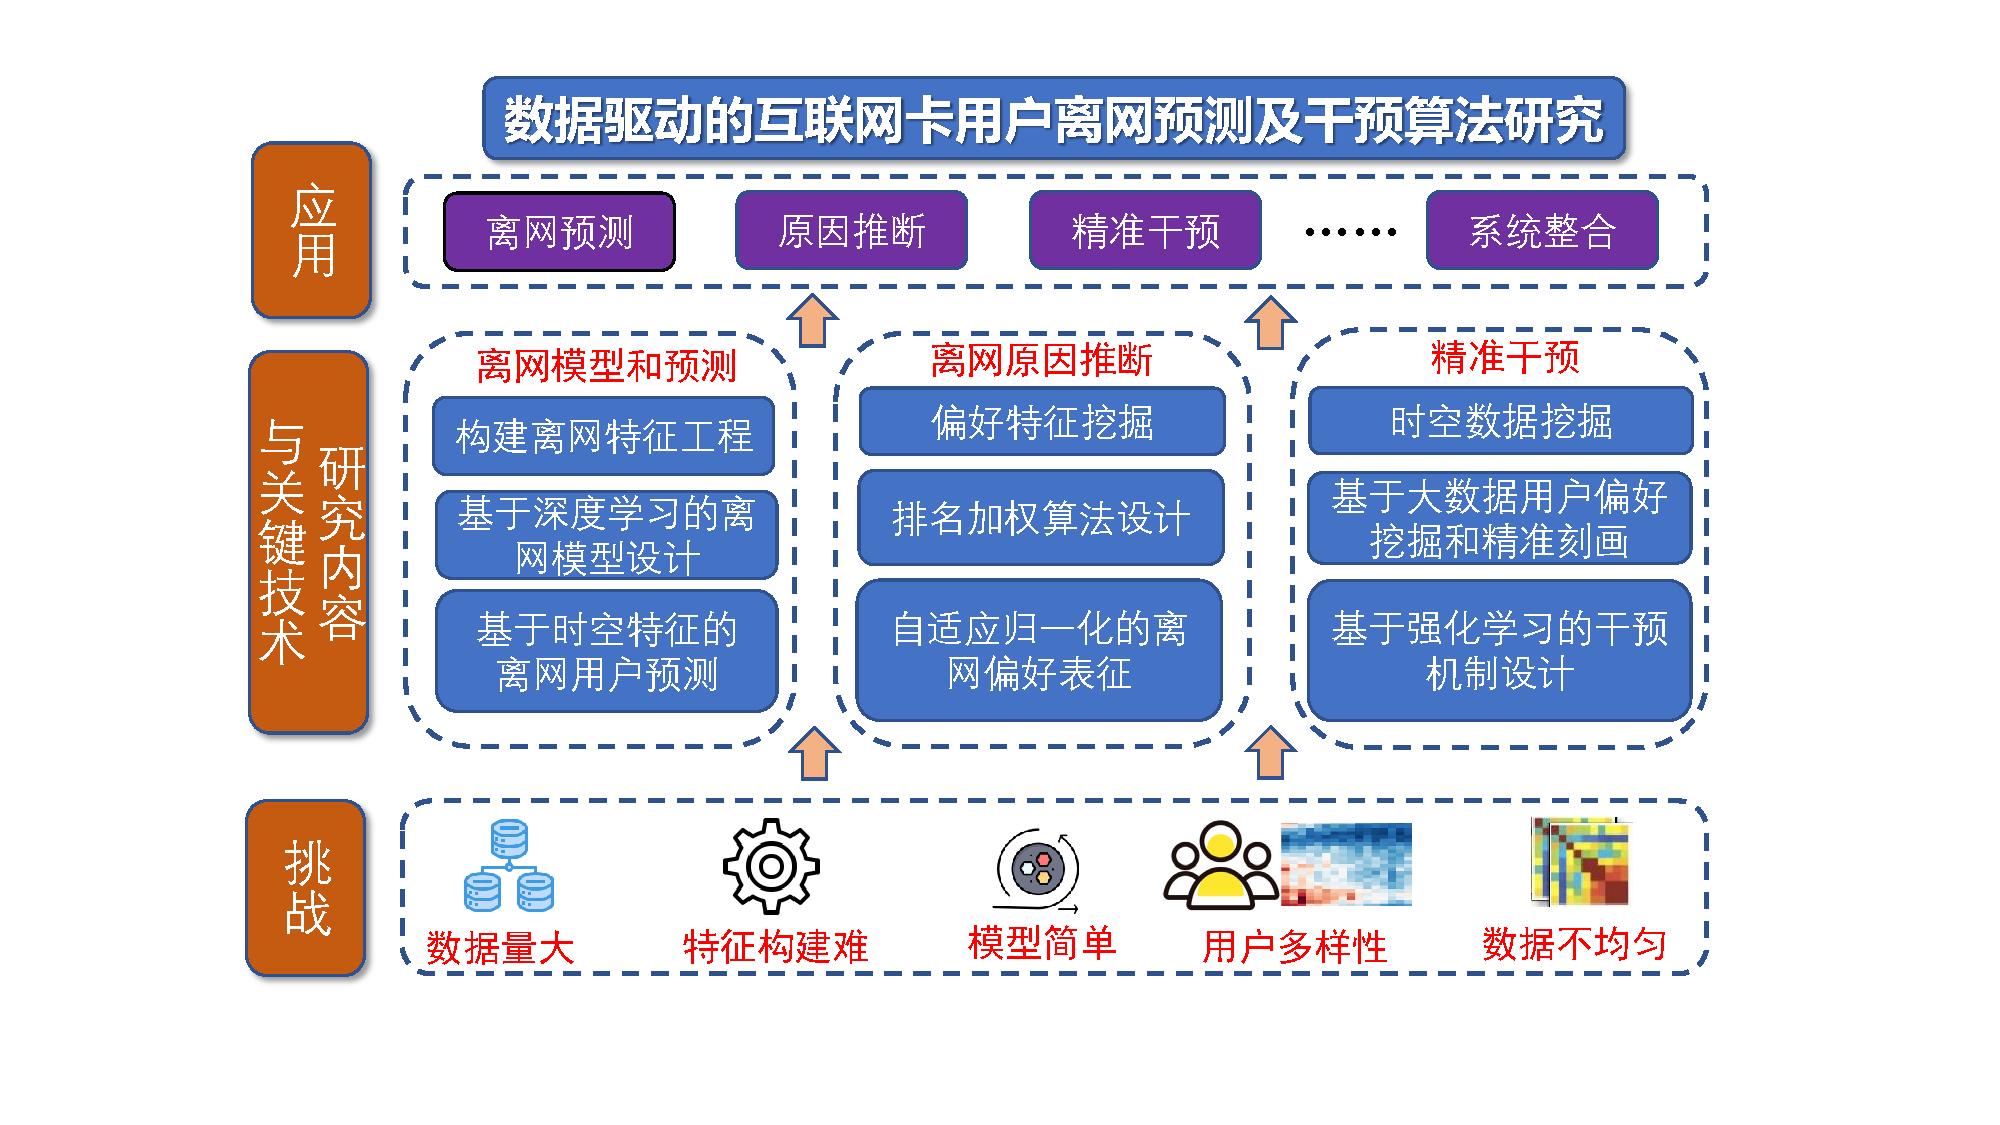
\includegraphics[width=1\textwidth]{Paper-Architecture_v1_1.pdf}
	\caption{论文组织架构图}
	\label{Fig:Paper_Architecture}
\end{figure}

\section{相关理论概述}
%\subsection{电信用户生命周期理论}%拉新、维护、干预
\subsection{用户画像}
\subsection{深度学习算法}
\subsubsection{卷积神经网络}
\subsubsection{循环神经网络}
\subsubsection{基于注意力机制的神经网络}
\subsection{强化学习算法}
\subsubsection{基于随机过程的多臂老虎机}
\subsubsection{基于上下文的多臂老虎机}
\subsection{本章小结}

\section{系统描述与问题建模}
\subsection{系统描述}
\subsubsection{离网用户预测模型}
\subsubsection{预离网用户偏好生成模型}
\subsubsection{预离网用户干预模型}
\subsection{问题建模}
\subsection{问题挑战}
\subsection{本章小结}

\section{用户数据分析和特征工程}
\subsection{平台描述}
\begin{figure}[hbt]
	\centering
	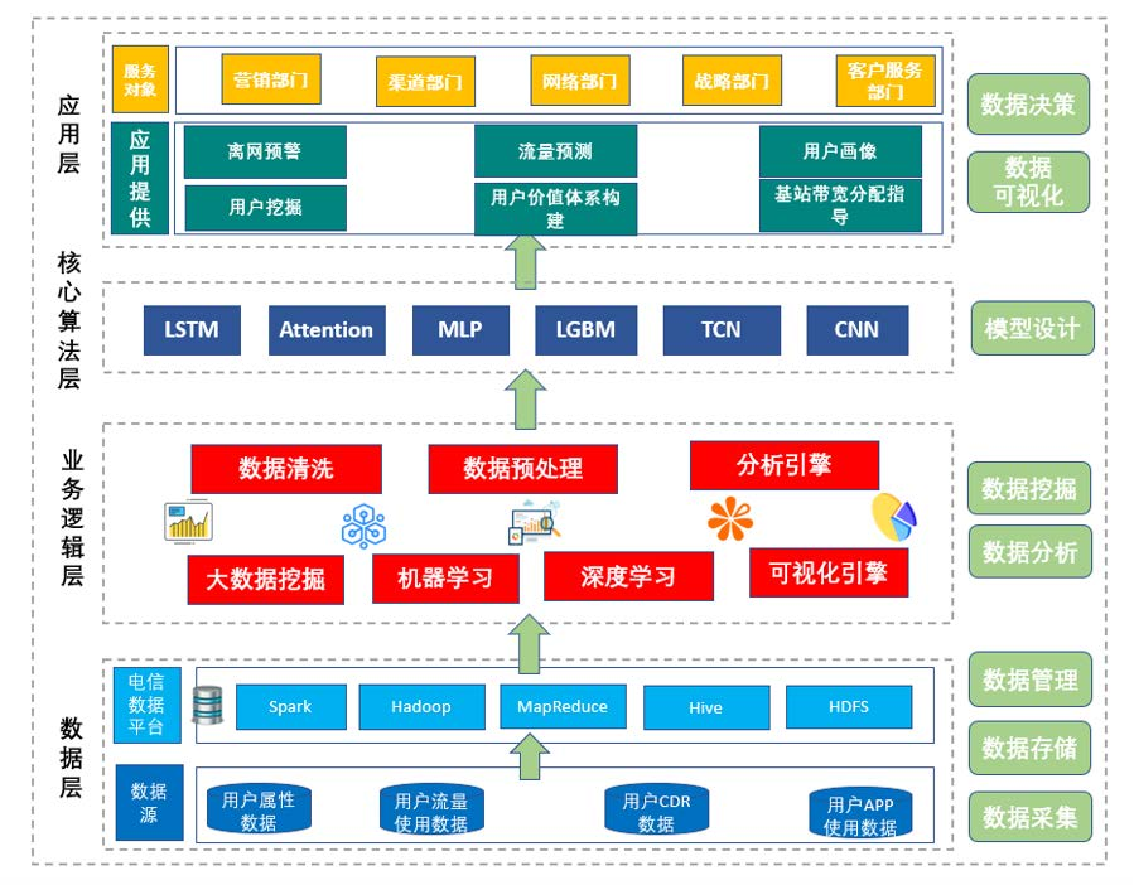
\includegraphics[width=1\textwidth]{Platform.pdf}
	\caption{大数据平台系统架构}
	\label{Fig:Data_Platform}
\end{figure}
在本章中, 我们会首先介绍平台架构,然后描述数据格式、规模等信息,接着进行了三个方面的数据分析,最后进行了相应的特征工程。
运营商们每天都会生产和存储巨量的数据,其中分为业务支持系统(BSS)和运营支持系统(OSS),这两者也构建了大数据平台的底层,从而用来提升业务和运营表现。具体来说,图\ref{Fig:Data_Platform}展示了流量运营商的大数据平台架构,其中包括数据层、业务逻辑层、核心算法层和应用层。在数据层中, 

\subsection{数据描述}
\begin{figure}[hbt]
	\centering
	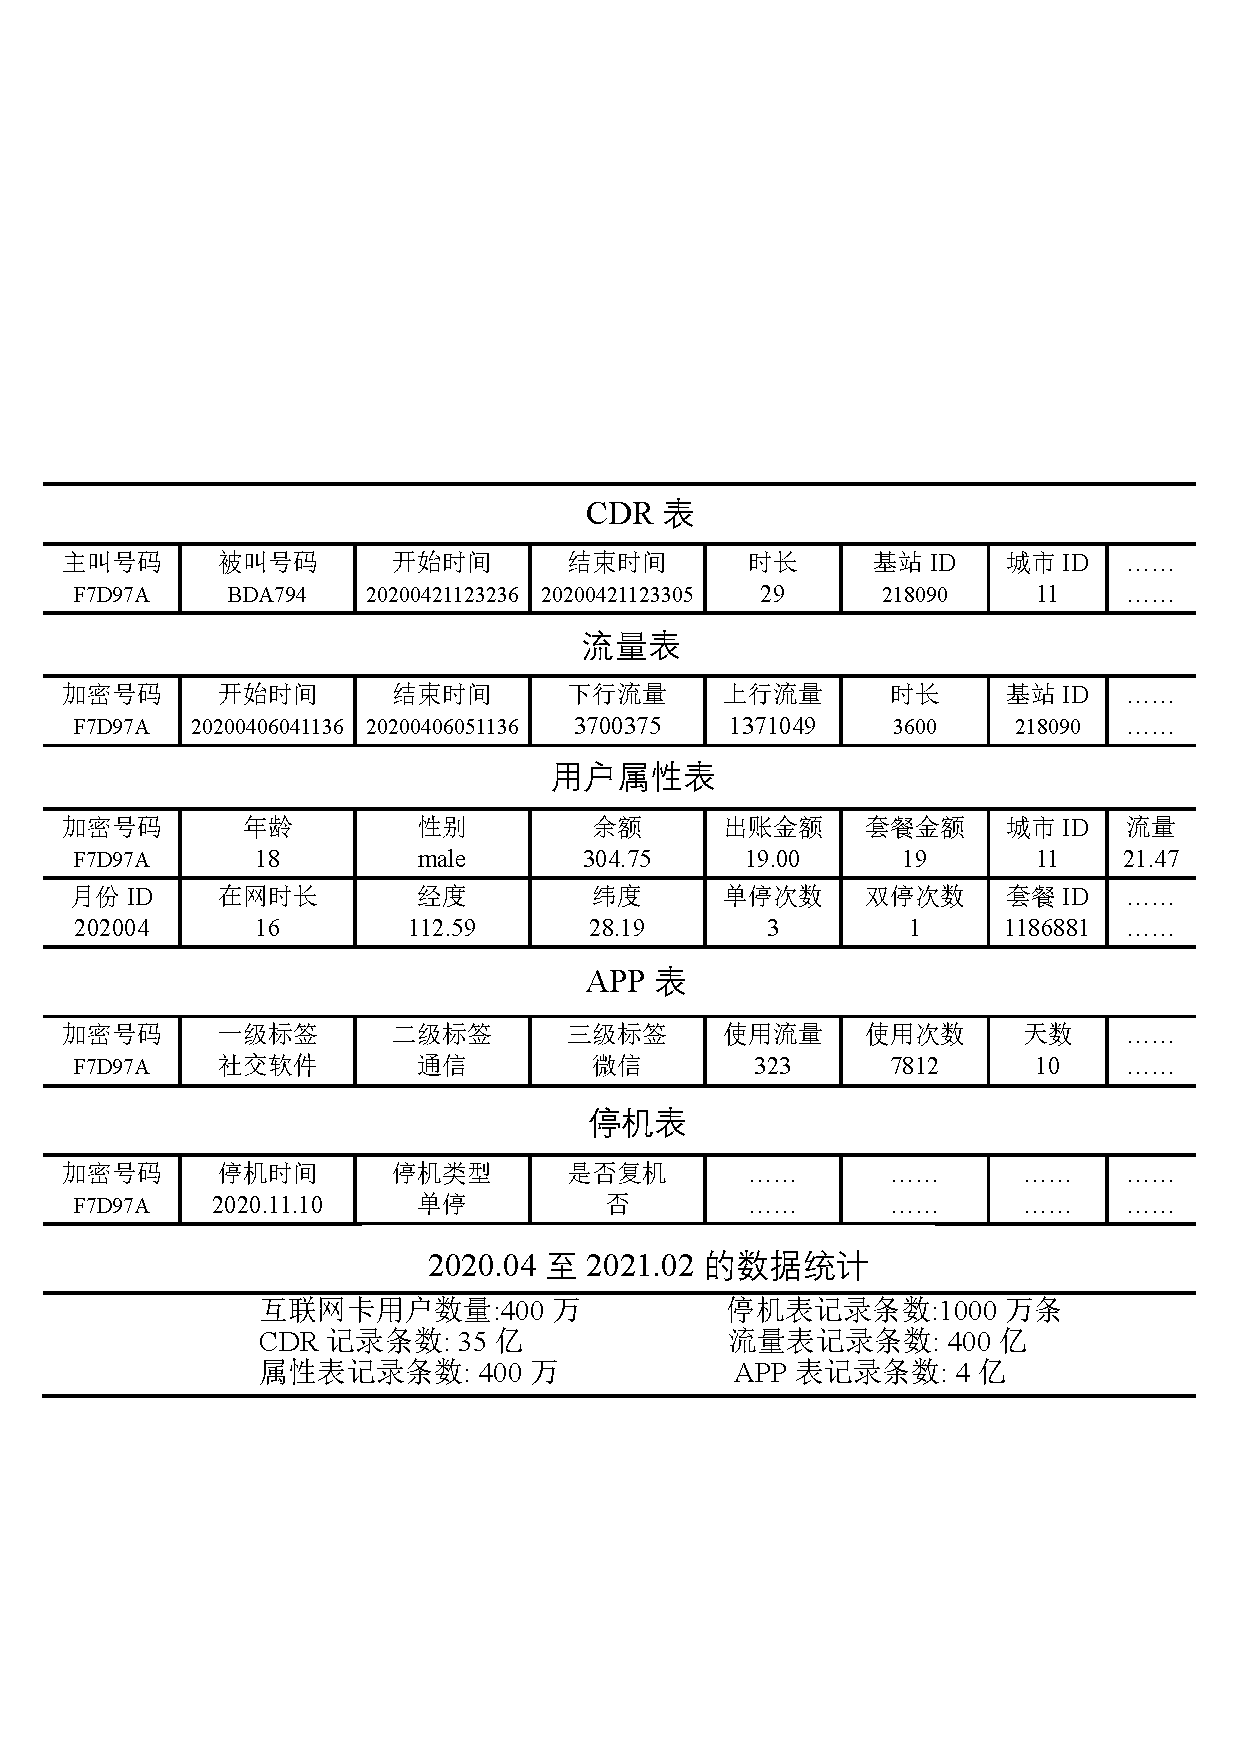
\includegraphics[width=1\textwidth]{Ms-Data-Description-ICCP_v1_1.pdf}
	\caption{用户侧数据描述}
	\label{Fig:User-Side-Data}
\end{figure}
首先, 我们来描述一下用户侧数据, 如图\ref{Fig:User-Side-Data}所示。\par
\textbf{时间范围.} 我们拥有从2020年4~6月,11月~12月和2021年1~2月的7个月的数据。\par
\textbf{用户类型.} 我们过滤掉了政企用户、家庭用户和其他用户,只留下互联网卡个人用户。\par
\textbf{数据规模.} 在这7个月的数据中,一共有400万的互联网卡个人用户,400万条以月为粒度的属性表记录,35亿条以次为粒度的CDR(通话细节记录)表记录,400亿条以次为粒度的流量表记录,4亿条以月为粒度的APP(应用程度)表记录, 1000万条以次为粒度的停机表记录。
其中属性表记录的为用户属性数据,而其他四个表记录的为用户行为数据,尤其是流量表和CDR表的数据尤为珍贵,能够刻画用户的序列行为。但是从另一方面来说,如此大量的数据也给数据分析和模型训练推理带来了极大的硬件资源、方法性能、时间压力。\par
\textbf{具体字段.}\par
\textbf{数据用途.} \par
\textbf{存储类型.} 这些数据主要是以HDFS\par

\begin{figure}[hbt]
	\centering
	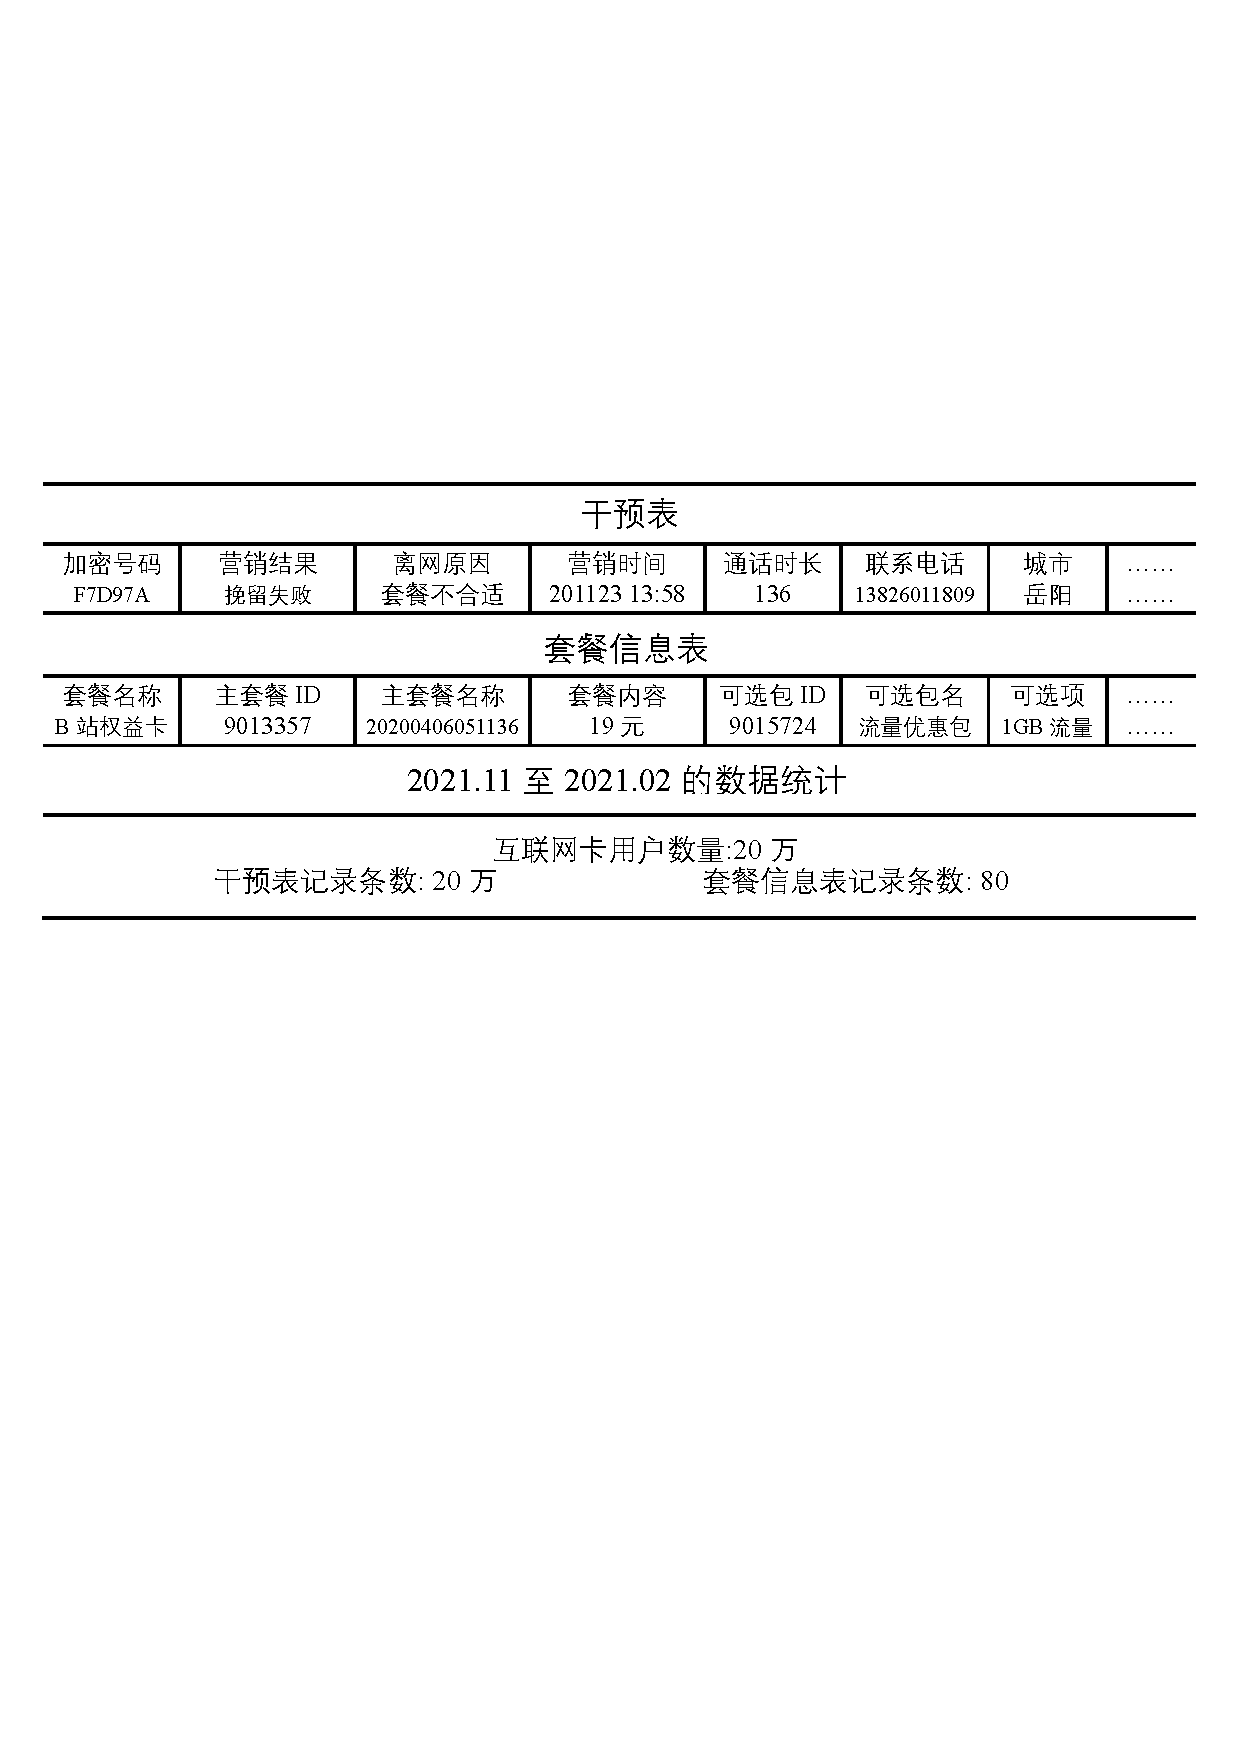
\includegraphics[width=1\textwidth]{Ms-Data-Description-ICSM_v2_1.pdf}
	\caption{物品侧数据描述}
	\label{Fig:Item-Side-Data}
\end{figure}
接着,我们来描述物品侧



\subsection{数据分析}
\subsubsection{用户静态属性分析}
\subsubsection{用户时序行为分析}
\subsubsection{用户异常行为分析}
\subsection{特征工程}
\subsubsection{静态特征工程}
\subsubsection{时序特征工程}
\subsection{本章小结}

\section{基于自注意力机制的互联网卡用户离网预测模型设计}
\subsection{系统描述与问题建模}
\subsection{基于PCA算法的特征降维算法}
\subsection{基于自注意力机制的嵌入向量表示}
\subsection{基于多层感知机的分类器设计}
\subsection{本章小结}

\section{预离网用户偏好生成算法设计}
\subsection{离网原因与偏好的相关性分析}
\subsection{离网偏好排名归一化}
\subsection{不可信用户过滤机制}
\subsection{本章小结}

\section{基于LinUCB的预离网用户干预模型设计}
\subsection{系统描述与问题建模}

\subsection{预离网用户偏好生成算法设计}
\subsubsection{离网原因与偏好的相关性分析}
\subsubsection{离网偏好排名归一化}
\subsubsection{不可信用户过滤机制}

\subsection{针对干预措施的特征工程}
\subsection{基于LinUCB的用户-干预措施匹配算法设计}
\subsubsection{动作空间}
\subsubsection{奖励机制设计}
\subsection{基于模拟干预结果机制的预训练}
\subsection{本章小结}

\section{实验评估与结果分析}
\subsection{实验设置}
\subsubsection{对比方案}
\subsubsection{评估指标}
\subsection{用户离网预测模型性能评估}
\subsection{预离网用户干预模型性能评估}
\subsection{参数影响}
\subsection{消融实验}
\subsection{本章小结}

\section{总结与展望}
\subsection{工作总结}
\subsection{未来工作展望}

\section{绪论}
\subsection{研究背景与意义}

目的是创建一个符合中南大学研究生学位论文(博士)撰写规范的LaTeX模板,解决学位论文撰写时格式调整的痛点。

已有珠玉在前,我们之所以还要重新造轮子,主要依据2022年4月18号学校下发的[《中南大学研究生学位论文撰写规范》中大研字【2022】8号] (http://oa.its.csu.edu.cn/Home/ReleaseMainText/9CFE8926B13143009D5EB424333AAD6C),重新修改了页面布局、字体类型和大小、标题内容,以期做到与 Word 模板尽可能的相似。\textbf{学校要求}:2022年起,申请博士、硕士学位的学位论文必须按新文件执行。主要修改如下:
\begin{itemize}
\item 按要求修订段落与各级标题间距;
\item 按要求修订中英文段落间距,章节间距,附录标题段落间距,研究成果及致谢标题间距,参考文献间距等;
\item 增加博士和硕士论文模板选项,只需要info.tex选择即可,方便使用;
\item 按新版撰写规范修改主要格式如下:修订目录章节标题间距;修订中英文段落间距;修订图片与表格标题的段落间距;
\item 按要求更新“学位论文版权使用授权书”;
\item 依据2022最新撰写规范修订封面和扉页-“封面”及“扉页”关于学科专业的表头更新为:一级学科/专业学位类别,二级学科/专业领域;
\item 依据专家意见修订定理和证明等环境,如”定理”使用小四黑体,编号随章节变化重新编号(如定理4-1),定理内容使用小四宋体,且内容行距与正文一致;”证明”无需编号,且以黑色小方块结尾;
\item 修订算法在每个章节重新编号问题;
\item 增加符号说明页和附录页(如果不需要,请在.cls文件对应处注释掉即可);
\item  增加参考文献按国标 gbt7714-2015要求,只核对了常用的图书、中英文期刊,会议格式,其余未常使用的未进行核对(如有问题请改回gbt7714-2005);
\item  修订多个子图Caption居中问题;
\item 依据专家意见调整成果与致谢部分间距,并增加目录中的点密度;
\item 按照图书馆最新要求(2020年12月份),去除目录中红色边框;
\item 增加页眉信息:中南大学博士论文与右侧的章节名保持一致,以及无需号章节名保持一致;
\item 增加中英文摘要至目录,并保持与章节名昨对其;
\item 参考文献完全依照国标 gbt7714-2005,修正了部分 Bug,提供了新的引用命令;
\item 按照最新版本要求,在声明扉页前后各增加一页空白页,保证装订单独成页;
\item 章节标题居中,并改成‘第1章’样式;
\item 目录中,将原章节标题换成‘第几章’样式,字体按要求加粗;
\item 中文摘要到目录结束用罗马数字编写页码,小五号Times New Roman,居中;
\item 增加插图索引和表格索引;
\item 所有的章节题目和中英文摘要均按要求修改字体和间距;
\end{itemize}

\subsection{主要研究工作}
\textbf{博士和硕士模板选择说明:}
\begin{itemize}
	\item 当前模板默认是博士,学术型。
	\item 如选择硕士模板,只需要将对应的content/info.tex文件中,选择$\setminus Doctorfalse$ \% 硕士学位论文,注释掉对应的博士模板就行。
	\item 学术型和专业型,盲审和正常版本,公开和涉密版本,均是同样操作;
	\item 其它模板,可以根据自己需要修改CSUthesis.cls文件。
\end{itemize}

(1) 提供图片插入示例。

(2) 提供表格插入示例。

(3) 提供公式插入示例。

(4) 提供参考文献插入示例。

\subsection{论文组织结构}

全文内容共六章,具体内容组织如下:

第一章为绪论。

第二章为图片插入示例。

第三章为表格插入示例。

第四章为公式插入示例。

第五章为参考文献插入示例。

第六章总结与展望,总结了本文的主要工作,展望了下一阶段的研究方向。

\clearpage

\section{图像布局}


\subsection{单图布局}



\textbf{单图布局如图\ref{F.csu_single}所示。}

\begin{figure}[hbt]
\centering
\includegraphics[width=0.5\textwidth]{csu.png}
\caption{单图布局示例}
\label{F.csu_single}
\end{figure}

\subsection{横排布局}

\textbf{横排布局如图\ref{F.csu_row}所示。}

\begin{figure}[!htb]
    \centering
    \begin{subfigure}[t]{0.24\linewidth}
    	\captionsetup{justification=centering} %子图caption居中
        \begin{minipage}[b]{1\linewidth}
        \includegraphics[width=1\linewidth]{csu.png}
         \caption{}
        \end{minipage}
    \end{subfigure}
    \begin{subfigure}[t]{0.24\linewidth}
    \captionsetup{justification=centering} %子图caption居中
        \begin{minipage}[b]{1\linewidth}
        \includegraphics[width=1\linewidth]{csu.png}
        \caption{}
        \end{minipage}
    \end{subfigure}
    \begin{subfigure}[t]{0.24\linewidth}
    	\captionsetup{justification=centering} %子图caption居中
        \begin{minipage}[b]{1\linewidth}
        \includegraphics[width=1\linewidth]{csu.png}
        \caption{}
        \end{minipage}
    \end{subfigure}
    \begin{subfigure}[t]{0.24\linewidth}
    	\captionsetup{justification=centering} %子图caption居中
        \begin{minipage}[b]{1\linewidth}
        \includegraphics[width=1\linewidth]{csu.png}
        \caption{}
        \end{minipage}
    \end{subfigure}
    \caption{横排布局示例}
    \label{F.csu_row}
\end{figure}



\subsection{竖排布局}
\textbf{竖排布局如图\ref{F.csu_col}所示。}

\begin{figure}[!htb]
    \centering
    \begin{subfigure}[t]{0.15\linewidth}
        \begin{minipage}[b]{1\linewidth}
        \includegraphics[width=1\linewidth]{csu.png}
        \caption{}
        \end{minipage}
    \end{subfigure}\\
    \begin{subfigure}[t]{0.15\linewidth}
        \begin{minipage}[b]{1\linewidth}
        \includegraphics[width=1\linewidth]{csu.png}
        \caption{}
        \end{minipage}
    \end{subfigure}
    \caption{竖排布局示例}
    \label{F.csu_col}
\end{figure}



\subsubsection{竖排多图横排布局}

\begin{figure}[!htb]
    \centering
    \begin{subfigure}[t]{0.13\linewidth}
    	\captionsetup{justification=centering} %子图caption居中
        \begin{minipage}[b]{1\linewidth}
        \includegraphics[width=1\linewidth]{csu.png} \vspace{-1ex} \vfill
        \includegraphics[width=1\linewidth]{csu.png}
         \caption{}
        \end{minipage}
    \end{subfigure}
    \begin{subfigure}[t]{0.13\linewidth}
    	\captionsetup{justification=centering} %子图caption居中
        \begin{minipage}[b]{1\linewidth}
        \includegraphics[width=1\linewidth]{csu.png} \vspace{-1ex} \vfill
        \includegraphics[width=1\linewidth]{csu.png}
        \caption{}
        \end{minipage}
    \end{subfigure}
    \caption{竖排多图横排布局}
    \label{F.csu_col_row}
\end{figure}

\textbf{竖排多图横排布局如图\ref{F.csu_col_row}所示。注意看(a)、(b)编号与图关系。}


\subsubsection{横排多图竖排布局}



\begin{figure}[!htb]
    \centering
    \begin{subfigure}[t]{0.3\linewidth}
    	\captionsetup{justification=centering} %子图caption居中
        \begin{minipage}[b]{1\linewidth}
        \includegraphics[width=0.45\linewidth]{csu.png}
        \includegraphics[width=0.45\linewidth]{csu.png}
        \caption{}
        \end{minipage}
    \end{subfigure}\\
    \begin{subfigure}[t]{0.3\linewidth}
    	\captionsetup{justification=centering} %子图caption居中
        \begin{minipage}[b]{1\linewidth}
        \includegraphics[width=0.45\linewidth]{csu.png}
        \includegraphics[width=0.45\linewidth]{csu.png}
        \caption{}
        \end{minipage}
    \end{subfigure}
    \caption{横排多图竖排布局,斜体emph \emph{A},A,斜体texit \textit{A}}
    \label{F.csu_row_col}
\end{figure}

\textbf{横排多图竖排布局如图\ref{F.csu_row_col}所示。注意看(a)、(b)编号与图关系。}

\subsection{本章小结}
本章示例图片布局。

\clearpage


\section{表格插入示例}

\begin{table}[htb]
  \centering
  \caption{表格为三线表斜体emph \emph{A},A,斜体texit \textit{A}}
  \label{T.example}
  \begin{tabular}{llllll}
  \toprule
    & \emph{A}A \textit{A}  & B  & C  & D  & E \\
  \midrule
1 	& 212 & 414 & 4 		& 23 & fgw	\\
2 	& 212 & 414 & v 		& 23 & fgw	\\
3 	& 212 & 414 & vfwe		& 23 & 嗯	\\
4 	& 212 & 414 & 4fwe		& 23 & 嗯	\\
5 	& af2 & 4vx & 4 		& 23 & fgw	\\
6 	& af2 & 4vx & 4 		& 23 & fgw	\\
7 	& 212 & 414 & 4 		& 23 & fgw	\\
\bottomrule

\end{tabular}
\end{table}

\textbf{表格如表\ref{T.example}所示,latex表格技巧很多,这里不再详细介绍。}



\clearpage

\section{算法示例}


\begin{algorithm}  
	\caption{Fourier-Mellin Based KCF}  
	\label{alg:A}  
	\hspace*{0.02in}{\bf Input:}
	Image $I$\\preprocessed kernelized template $T_\kappa$\\
	\hspace*{0.02in}{\bf Output:} 
	scale $\sigma$, angle $\theta$ relation between $I$ and $T$ 
	
	\begin{algorithmic}[1] 
		\STATE{fourier transform: $F=\mathcal{F}(I)$}
		\STATE {high pass filter: $F_h=\mathcal{H}(F)$\\$\mathcal{H}(x,y)=(1.0-cos(\pi x)cos(\pi y))(2.0-cos(\pi x)cos(\pi y))$}
		\STATE {log-polar transform: $F_{lp}=\mathcal{L}(F_h)$}
		\STATE {apply kernel function: $F_\kappa=\mathcal{K}(F_{lp})$}
		\STATE {phase correlation: $(\Delta x, \Delta y)=\mathcal{C}(F_\kappa, T_\kappa)$}
		\STATE {resolove scale and rotation:\\
			$\theta=\alpha \Delta x$, $\sigma=log(\Delta y)$\\
			where $\alpha$ is translation factor of pixel translation on fourier domain and polar angle on origin image
		}
	\end{algorithmic}  
\end{algorithm}


  \begin{algorithm}
	\caption{算法示例}
	\label{alg:SPSH01}
	\renewcommand{\algorithmicrequire}{\textbf{Input:}}
	\renewcommand{\algorithmicensure}{\textbf{Output:}}
	
	\begin{algorithmic}[1]
		\REQUIRE 相关输入。。。。
		
		\ENSURE 相关输出。。。
		
		\STATE 算法描述  % 只占用一个行号
		\FOR{$i \gets 1\cdots N$}
		\STATE 算法描述
		\FOR{\textbf{each} $j \gets 1\cdots K$}
		\STATE 算法描述
		\ENDFOR
		\ENDFOR
		\REPEAT
		\REPEAT
		\STATE 令$\tau\gets\tau+1$
		\UNTIL 内循环迭代终止条件
		\STATE 。。。
		\UNTIL 外循环迭代终止条件
	\end{algorithmic}
\end{algorithm}

\textbf{如算法\ref{alg:A}所示,latex算法技巧很多。按需调整,这里不再详细介绍。}

\clearpage

\section{公式、定理、证明插入示例}

\begin{flalign}
\text{P1: } &\min_{\eta,R_u>0,R_d>0}\big\{ T_{\text{latency}}(\eta,R_u,R_d)\big\}  \\
&\text{s.t. }   0 \leq \eta \leq 1 \label{P1C1} 
\end{flalign}

\textbf{公式插入示例如公式(\ref{E.example})所示。}

\begin{equation}
\gamma_{x}=
\left\{
  \begin{array}{lr}
  0, & {\rm if}~~\;|x| \leq \delta \\
  x, & {\rm otherwise}
  \end{array}
\right.
\label{E.example}
\end{equation}

\begin{flalign}
&\text{P1:} \max_{\bigg\{\substack{P_{m,i},P_{n,i}\\
		q_{m,i},q_{n,i}\\ \forall n,m,i}\bigg\}}\big[R_{\text{sum}}(P_{m,i},P_{n,i},q_{m,i},q_{n,i},\forall n,m,i)\big],  \\
& \text{s.t.}~~q_{m,i}\in(0,1), q_{n,i}\in(0,1), \forall n,m,i, \label{allocons1} \\
& \hspace{1.5em} ~0\leq \sum_{i=1}^Rq_{n,i}P_{n,i}\leq P_n^{sum}, \forall n, \label{powercons1}  \\ 
& \hspace{1.5em} ~0\leq \sum_{i=1}^Rq_{m,i}P_{m,i}\leq P_m^{sum}, \forall m, \label{powercons2} \\ 
& \hspace{1.5em} ~\sum_{i=1}^Rq_{n,i}\leq 1,\sum_{i=1}^Rq_{m,i}\leq 1,\forall m,n, \label{RBcons} \\ 
& \hspace{1.5em} ~\sum_{n=1}^Nq_{n,i}\leq 1,\sum_{m=1}^Mq_{m,i}\leq 1,\forall i, \label{RBcons2} \\
& \hspace{1.5em} ~C_{m,BS,i}(P_{m,i},q_{m,i})\geq\varepsilon_{m,i},\forall m, \label{capcons}
\end{flalign}


  %%%%%%%%%%%%%% 示例 %%%%%%%%%%%%%%%%
公式子编号示例:
\begin{subequations}\label{Eq.(3-4)}
	\renewcommand{\theequation}{\theparentequation-\alph{equation}} % 定义编号方式
	\begin{align}
		&\varphi_{n,t}\in\left\{0,1\right\}, \forall n\in\mathcal{N}, t\in\mathcal{N}_{\mathrm{t}}, \label{Eq.(3-4a)} \\
		&\varphi_{n,t}\in\left\{0,1\right\}, \forall n\in\mathcal{N}, t\in\mathcal{N}_{\mathrm{t}}, \label{Eq.(3-4b)} \\
		&\varphi_{n,t}\in\left\{0,1\right\}, \forall n\in\mathcal{N}, t\in\mathcal{N}_{\mathrm{t}}, \label{Eq.(3-4c)}
	\end{align}
\end{subequations}

其中,公式\ref{Eq.(3-4a)}表示。

\begin{equation}    
	H_{j}= \mathrm{Concat}(\mathrm{GAP}({F}_{j}),\mathrm{GMP}({F}_{j})),
\end{equation}
\begin{equation}    
	\tilde{H}_{j-1,j}= \mathrm{Concat}(H_{j-1},H_{j}),j=5,
\end{equation}
\begin{equation}    
	p_c^{(i)}=\mathrm{Softmax}(\boldsymbol{P}_\theta(\tilde{H}_{j-1,j})),
\end{equation}

  %%%%%%%%%% 示例 %%%%%%%%%%%5
定理和证明环境说明:如”定理”使用小四黑体,编号随章节变化重新编号(如定理4-1),定理内容使用小四宋体,且内容行距与正文一致;”证明”无需编号,且以黑色小方块结尾。

\begin{theorem}\label{theorem1}
	\setlength{\baselineskip}{20pt}         % 基准行间距
	\renewcommand{\baselinestretch}{1.0}   % 几倍行间距
	开始定理。。。
\end{theorem}

\begin{proof*} %% 证明不编号
	\setlength{\baselineskip}{20pt}         % 基准行间距
	\renewcommand{\baselinestretch}{1.0}   % 几倍行间距
	开始证明。。。
	$\hfill\blacksquare$ %% 以黑方块结尾
\end{proof*}

\clearpage

\section{参考文献插入示例}

LaTeX\cite{lamport1994latex}插入参考文献最方便的方式是使用bibliography\cite{pritchard1969statistical},大多数出版商的论文页面都会有导出bib格式参考文献的链接,建议使用Jabref管理参考文献,把每个文献的bib放入``thesis-references'',然后用bibkey即可插入参考文献。

中文文献\cite{zh-book-1},注意手动编辑bibkey为英文的即可。

可以将文献标注为右上角\citess{shiweisong2019},只需要在现有的cite后加“ss”即可。

英文会议\cite{Kraus2021Current}, \cite{WuYangLuEtAl2021}.

英文期刊\cite{LuoZengYuanEtAl2016}, \cite{Wu2022Boosting}.


\textbf{特别强调:}从Google下载的bib也不一定全是对的,如发现有信息缺失,请下载原文核对。比如已发表的期刊,要包保证年、卷、标。

\textbf{注意:}如发现替换后的参考文献没有更新,请删除主文件夹下xxx.bbl文件,重新编译即可。

\clearpage


\section{总结与展望}

\noindent{纯数字编号}
\begin{enumerate}
 \item XXXXXXXXXX
 \label{item1}
 \item XXXXXXXXXX
 \item XXXXXXXXXX
\end{enumerate}
罗马编号
\begin{enumerate}[label=(\roman*)]
 \item XXXXXXXXXX
 \label{item2}
 \item XXXXXXXXXX
 \item XXXXXXXXXX
\end{enumerate}
括号编号
\begin{enumerate}[label=(\arabic*)]
 \item XXXXXXXXXX
 \label{item3}
 \item XXXXXXXXXX
 \item XXXXXXXXXX
\end{enumerate}
半括号编号
\begin{enumerate}[label=\arabic*)]
 \item XXXXXXXXXX
 \label{item4}
 \item XXXXXXXXXX
 \item XXXXXXXXXX
\end{enumerate}
小字母编号
\begin{enumerate}[label=\alph*)]
 \item XXXXXXXXXX
 \label{item5}
 \item XXXXXXXXXX
 \item XXXXXXXXXX
\end{enumerate}

引用测试,正如\ref{item1}、\ref{item2}、\ref{item3}、\ref{item4}、\ref{item5}所示

\subsection{工作展望}
手动编号 %(不推荐,无法被交叉引用)
\par
本课题针对XX,鉴于XXX,对XX进行了提高,但是XXX,所以有如下XX:

(1)目前XX虽然XX,但是XX仍然XX,所以XX仍然是一个值得XX的问题。

(2)随着XX,XX具有XX的问题,仍值得进一步XX。

(3)本课题在XX有了XX,但是XX的XX还存在XX,所以XX。


\clearpage

	}
	
	%%%%%%%%%%%%%%%%%%%%%%%%%%%%%%%%%%%%%%%%%%%%%%%%%%
	% 临时标签,用于编译时追踪正文末尾
	%%%%%%%%%%%%%%%%%%%%%%%%%%%%%%%%%%%%%%%%%%%%%%%%%%
	
	%%%%%%%%%%%%%%%%%%%%%%%%%%%%%%%%%%%%%%%%%%%%%%%%%%
	% 后续内容,标题三号黑体居中,章节无编号
	% --------------------------------------------%
	
	% https://www.zhihu.com/question/29413517/answer/44358389 %
	% 说明如下:
	% secnumdepth 这个计数器是 LaTeX 标准文档类用来控制章节编号深度的。在 article 中,这个计数器的值默认是 3,对应的章节命令是 \subsubsection。也就是说,默认情况下,article 将会对 \subsubsection 及其之上的所有章节标题进行编号,也就是 \part, \section, \subsection, \subsubsection。LaTeX 标准文档类中,最大的标题是 \part。它在 book 和 report 类中的层级是「-1」,在 article 类中的层级是「0」。这里,我们在调用 \appendix 的时候将计数器设置为 -2,因此所有的章节命令都不会编号了。不过,一般还是会保留 \part 的编号的。所以在实际使用中,将它设置为 0 就可以了。
	
	% 在修改过程中请注意不要破环命令的完整性
	
	\renewcommand\appendix{\setcounter{secnumdepth}{-2}}
	\appendix
	
	% 主文件有代码去掉页眉章节编号的“.”,但这会因为bug导致无编号章节显示一个错误编号,所以这里在无编号章节之前再次重定义sectionmark。
	\renewcommand{\sectionmark}[1]{\markboth{#1}{#1}}
	\renewcommand{\subsectionmark}[1]{\markright{\leftmark}}
	\renewcommand{\subsubsectionmark}[1]{\markright{\leftmark}}
	
	% section 标题从这里往后改为三号黑体居中
	\titleformat{\section}{\centering \zihao{3} \bfseries \heiti}{\thesection}{1em}{}
	\titlespacing*{\section} {0pt}{18pt}{32pt}
	
	% \section{参考文献} % bibliography会自动显示参考文献四个字
	
	% \nocite{*} % 该命令用于显示全部参考文献,即使文中没引用
	% cls文件中已经引入package,这里不需要调用 \bibliographystyle 了。
	% \bibliographystyle{gbt7714-2005} 
	{~}
	\vspace{18pt}
	\phantomsection                                      %% 解决目录中超链接地址错误问题
	\addcontentsline{toc}{section}{参考文献} % 由于参考文献不是section,这句把参考文献加入目录
	\zihao{-4} \setmainfont{Times New Roman}
	\setlength{\baselineskip}{20pt}         % 基准行间距 
	\bibliographystyle{gbt7714-2015-little} 
	\bibliography{thesis-references}
	
	\clearpage
	% 附录
	
	\titleformat{\section}{\centering \zihao{3} \bfseries \heiti}{\thesection}{1em}{}
	\titlespacing*{\section} {0pt}{18pt}{32pt}
	\titleformat{\subsection}{\zihao{-4} \songti}{\thesubsection}{1em}{}
	\titlespacing*{\subsection} {2em}{0pt}{0pt}
	\titleformat{\subsubsection}{\zihao{-4} \songti}{\thesubsubsection}{1em}{}
	\titlespacing*{\subsubsection} {2em}{0pt}{0pt}
	
	%{~}
%\vspace{18pt}
%\section{附录A (附录名称 )(三号黑体,加粗)(必要时)} % 无章节编号
%
%附录正文…
%…(格式参考正文)。
%换行示例
%。

%\newpage
%
%{~}
%\vspace{18pt}
%\section{附录B (附录名称 )(三号黑体,加粗)(必要时)} % 无章节编号
%
%附录正文…
%…(格式参考正文)。
%换行示例
%。

	
	\clearpage
	% 研究成果和致谢
	
	\titleformat{\section}{\centering \zihao{3} \bfseries \heiti}{\thesection}{1em}{}
	\titlespacing*{\section} {0pt}{18pt}{32pt}
	\titleformat{\subsection}{\zihao{-4} \songti}{\thesubsection}{1em}{}
	\titlespacing*{\subsection} {2em}{0pt}{0pt}
	\titleformat{\subsubsection}{\zihao{-4} \songti}{\thesubsubsection}{1em}{}
	\titlespacing*{\subsubsection} {2em}{0pt}{0pt}
	
	%!TEX root = ../csuthesis_main.tex

{~}
\vspace{18pt}
\section{攻读学位期间主要的研究成果} % 无章节编号

\ifblindreview
% \noindent
% (盲审隐去作者相关具体信息)
\fi
\vspace{11pt}
\subsection*{一、学术论文}

\ifblindreview

% \noindent
% 第一作者:JCR 1 区 x 篇,会议 x 篇 \\{}
% 第二作者:JCR 1 区 x 篇,3 区 x 篇,4 区 x 篇,EI x 篇 

% \noindent
% 投稿状态: 
% IEEE Transactions on Image Processing 1篇(under review)\\{}
% IEEE Transactions on Circuits and Systems for Video Technology 1 篇(Accept with Minor Revision)

% 学位办老师要求用如下这种几乎算是单盲的格式,我也木有办法……
\subsubsection*{已录用/检索论文}
%\noindent
%第一作者:
%\begin{enumerate}[label={[\arabic*]},itemindent=2em,wide]
%	\item CSU Latex Template[J]. CSU player: 1(1):1-10. {\bfseries \heiti(SCI 录用,JCR 1 区)}
%	\item CSU Latex Template[J]. CSU player: 1(1):1-10. {\bfseries \heiti(SCI 检索,JCR 2 区)}
%\end{enumerate}
%第二作者:
%\begin{enumerate}[label={[\arabic*]},itemindent=2em,wide]
%	\item CSU Latex Template[J]. CSU player: 1(1):1-10. {\bfseries \heiti(SCI 检索,JCR 1 区)}
%	\item CSU Latex Template[J]. CSU player: 1(1):1-10. {\bfseries \heiti(SCI 检索,JCR 2 区)}
%\end{enumerate}
第五作者:
\begin{enumerate}[label={[\arabic*]},itemindent=2em,wide]
	\item Characterizing Internet Card User Portraits for Efficient Churn Prediction Model Design[J]. IEEE Transaction on Mobile Computing, 2023. {\bfseries \heiti(SCI 检索,JCR 1 区)}
	%	\item Director, \textbf{Daxia Mou}, Someone, Someother. XXXXXX[J]. Transactions on Image Processing. {\bfseries \heiti(SCI Under Review,JCR 1 区)}
	%	\item Director, \textbf{Daxia Mou}, Someone, Someother. XXXXXX[J]. Transactions on Circuits and Systems for Video Technology. {\bfseries \heiti(SCI Under Review,JCR 1 区)}
\end{enumerate}
%\noindent
%\subsubsection*{投稿状态论文}
%%\noindent
%第一作者:
%\begin{enumerate}[label={[\arabic*]},itemindent=2em,wide]
%	\item CSU Latex Template. XXX Transactions on CSU player. {\bfseries \heiti(SCI Under Review,JCR 1 区)}
%\end{enumerate}
%第二作者:
%\begin{enumerate}[label={[\arabic*]},itemindent=2em,wide]
%	\item CSU Latex Template. XXX Transactions on CSU player. {\bfseries \heiti(SCI Under Review,JCR 1 区)}
%	\item CSU Latex Template. XXX Transactions on CSU player. {\bfseries \heiti(SCI Under Review,JCR 2 区)}
%\end{enumerate}


\else
% 标准版本
\begin{enumerate}[label={[\arabic*]},itemindent=2em,wide]
	\item Fan Wu, Feng Lyu, Ju Ren, Peng Yang, \textbf{Kai Qian}, Shijie Gao, Yaoxue Zhang. Characterizing Internet Card User Portraits for Efficient Churn Prediction Model Design[J]. IEEE Transaction on Mobile Computing: 1(1):1-10. {\bfseries \heiti(SCI 检索,JCR1区)}
%	\item Director, \textbf{Daxia Mou}, Someone, Someother. XXXXXX[J]. Transactions on Image Processing. {\bfseries \heiti(SCI Under Review,JCR 1 区)}
%	\item Director, \textbf{Daxia Mou}, Someone, Someother. XXXXXX[J]. Transactions on Circuits and Systems for Video Technology. {\bfseries \heiti(SCI Under Review,JCR 1 区)}
\end{enumerate}
\fi

\vspace{22pt}
\subsection*{二、发明专利}
\ifblindreview
发明专利3项,其中2项已授权,1项已受理
\begin{enumerate}[label={[\arabic*]},itemindent=2em,wide]
	\item 导师第一发明人,本人第二发明人. 基于深度学习的用户流失预测方法及系统. 2022-11-01. 已授权.
	\item 导师第一发明人,本人第二发明人. 基于用户画像的互联网卡用户流失预测方法及系统. 2021-11-29. 已受理.
	\item 第五发明人. 一种数据驱动的互联网卡用户价值分类方法设备及介质. 2023-03-14. 已授权.
\end{enumerate}
\else
发明专利3项,其中2项已授权,1项已公开
\begin{enumerate}[label={[\arabic*]},itemindent=2em,wide]
	\item 吕丰,\textbf{钱凯},吴帆,任炬,张尧学. 基于深度学习的用户流失预测方法及系统. 申请号:CN2021112951915,授权公告号:CN 114022202 B
	\item 吕丰,\textbf{钱凯},吴帆,任炬,张尧学. 基于用户画像的互联网卡用户流失预测方法及系统. 申请号:2021112981395,公开号:CN 113962160 A
	\item 高世杰,张永敏,王姗姗,周杰钰,\textbf{钱凯}. 一种数据驱动的互联网卡用户价值分类方法设备及介质:ZL 202211513076.5[P]. 授权公告号:CN 115563555 B
\end{enumerate}
\fi

\ifblindreview
\else

\vspace{22pt}
%\subsection*{三、主持和参与的科研项目}
%\begin{enumerate}[label={[\arabic*]},itemindent=2em,wide]
%	\item 国家自然科学基金面上项目《XXXXXXXXXXXX》, 项目编号:XXXXXXXX,参与.
%\end{enumerate}

% {~}
\vspace{22pt}
\subsection*{三、个人获奖情况}
%\noindent
\begin{enumerate}[label={[\arabic*]},itemindent=2em,wide]
	\item 2020年度中南大学研究生一等奖学金
	\item 2021年度中南大学研究生二等奖学金
	\item 2022年度中南大学研究生二等奖学金
\end{enumerate}
\fi

%\newpage

\ifblindreview
\else

{~}
\vspace{18pt}

\newpage

\section{致谢} % 无章节编号
	白驹过隙,日月如梭,不知不觉间已经在透明计算实验室度过了三年难忘的研究生生活了。其中酸甜苦辣,百般滋味,只有自己知晓,不足为外人道也。但是,我今天能成功地取得硕士学位,离不开家人和以下老师,朋友的一贯支持和有力帮助。\par
	首先,我想感谢我的恩师,吕丰教授。在透明计算实验室的三年多的研究生生活中,吕老师不遗余力地指导我进行科研课题的研究,教授我解决问题的通用范式,身体力行地为我树立想要从事科研应当学习的榜样。在每次的组会讨论,外出谈判中,我都能从吕老师身上学习到了更加准确的思维逻辑和为人处世。\par
	其次,我想感谢实验室的吴帆、刘彤、周杰钰师兄和卢华丽、段思婧师姐,他们作为博士师兄、师姐,首先给了在科研和生活中非常多的指导以及帮助,并且他们身上刻苦钻研的科研精神和求实务真的科研态度深深地激励了我。\par
	然后,我想感谢实验室的同门,包括肖飞、高世杰、王艺锋、何骁豪、刘佳璇、张静,还有赵张梦茹、王姗姗、孟陈莹、唐程等师弟师妹们,他们每个人身上都有各自的闪光点和才华,和他们的朝夕相处中,我不仅感受到了蓬勃的青春,而且被处处的真情所感动,大家都十分团结,互帮互助,在一起时充满了欢声笑语。只可惜时不我待,我不得不和他们挥手告别。但是往昔的情谊都留在心中,不必多说。\par
	最后,我想感谢我的家人们,包括我的爸爸、妈妈、爷爷、奶奶、外公、外婆等,在我外出求学的第5到7个年头,包括之后的8到12个年头,无论我提出什么要求,只要是我自己愿意的,他们都无条件地支持我,并且及时地给予我物质上的支持和精神的援助。他们对我的爱,我也都深深铭刻在心中,而我也将我的实际行动回报他们对我的爱。\par
	最后的最后,感谢所有花时间阅读我硕士学位的老师、同学和朋友们,你们的意见和建议将使我变得更好。希望在下一个四年,你们能看到我更加优秀的博士学位论文。言尽于此,我继续去科研了。


% 重新设置正文行间距,因为前置部分设置时候行间距被改过
\renewcommand*{\baselinestretch}{1.0} % 几倍行间距
\setlength{\baselineskip}{20pt} % 基准行间距

%作者对给予指导、各类资助和协完成研究工以及提供种论文有 作者对给予指导、各类资助和协完成研究工以及提供种论文有 利条件的单位及个人表示感谢。
%
%致谢应实事求是,切忌浮夸与庸俗之词 。

\newpage
\fi

	
	
\end{document}
